\section{Modelo de Mezcla Gaussiana} \label{sec_GMM}

Do Chuong y Batzoglou nos indican, en su artículo \textit{What is the expectation maximization algorithm?} [\ref{ChuongBatzoglou}], que el algoritmo de maximización de la esperanza (EM) es una generalización natural de la estimación por máxima verosimilitud. Ésto para el caso en donde se tiene información incompleta.

Los parámetros iniciales se toman de los datos con ello se obtienen unos parámetros finales que se convierten en los parámetros de la siguiente iteración. Así sucesivamente.

\url{https://www.youtube.com/watch?v=REypj2sy_5U&ab_channel=VictorLavrenko}

\url{https://www.youtube.com/watch?v=iQoXFmbXRJA&ab_channel=VictorLavrenko}

\url{https://www.youtube.com/watch?v=pYxNSUDSFH4&ab_channel=StatQuestwithJoshStarmer}


 The goal of the maximum likelihood is to find the optimal way to fit a distribution to the data:
 
\url{https://www.youtube.com/watch?v=XepXtl9YKwc&ab_channel=StatQuestwithJoshStarmer}


%\begin{figure}[H]
%\centering
%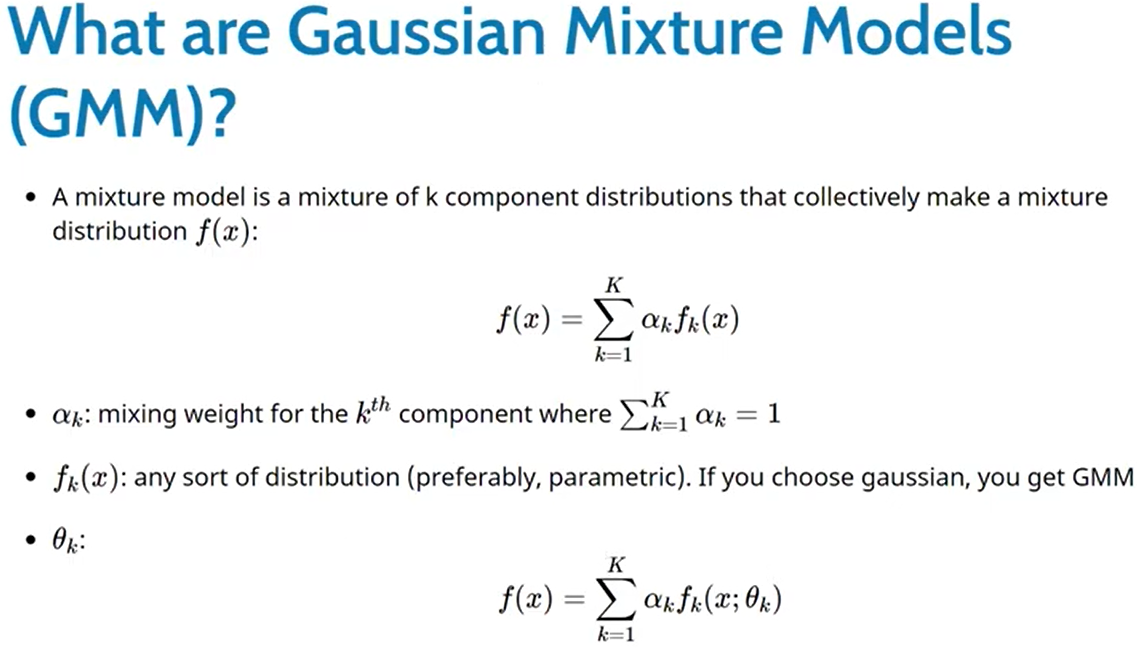
\includegraphics[scale = 0.5]{GMM_1} %width=\textwidth
%\caption{\textit{GMM 1}}
%\end{figure}
%
%\begin{figure}[H]
%\centering
%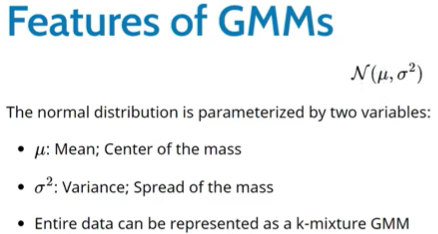
\includegraphics[scale = 0.5]{GMM_2} %width=\textwidth
%\caption{\textit{GMM 2}}
%\end{figure}
%
%\begin{figure}[H]
%\centering
%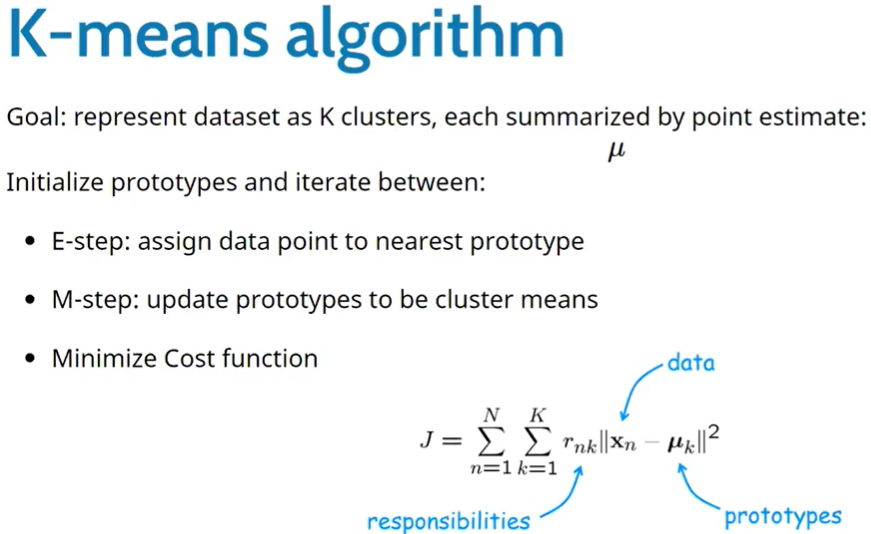
\includegraphics[scale = 0.5]{GMM_3} %width=\textwidth
%\caption{\textit{GMM 3}}
%\end{figure}
%
%\begin{figure}[H]
%\centering
%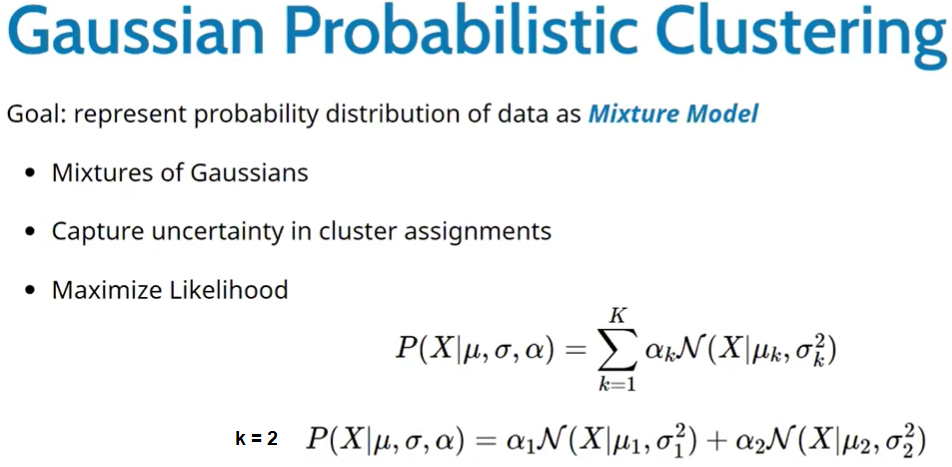
\includegraphics[scale = 0.5]{GMM_4} %width=\textwidth
%\caption{\textit{GMM 4}}
%\end{figure}
%
%\begin{figure}[H]
%\centering
%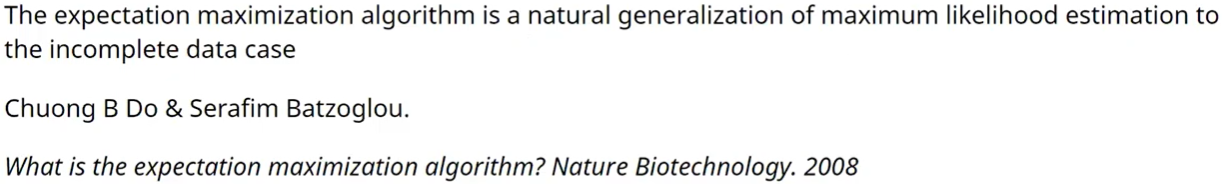
\includegraphics[scale = 0.5]{GMM_5} %width=\textwidth
%\caption{\textit{GMM 5}}
%\end{figure}
%
%\begin{figure}[H]
%\centering
%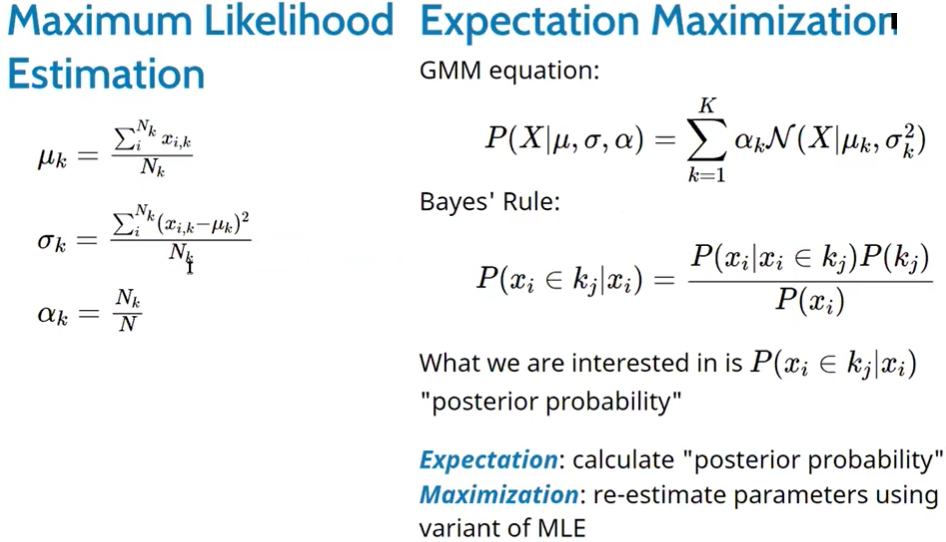
\includegraphics[scale = 0.5]{GMM_6} %width=\textwidth
%\caption{\textit{GMM 6}}
%\end{figure}
%
%\begin{figure}[H]
%\centering
%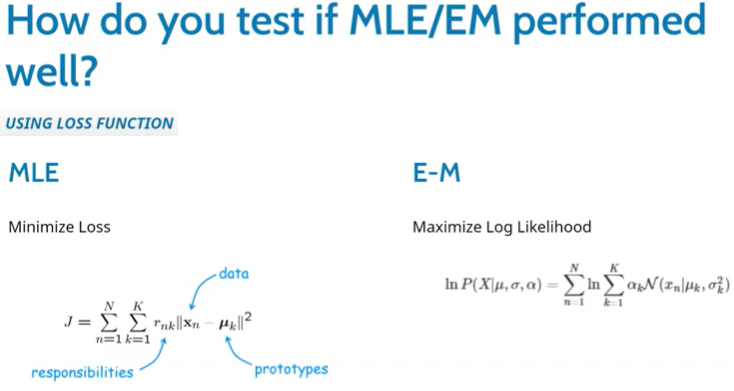
\includegraphics[scale = 0.5]{GMM_7} %width=\textwidth
%\caption{\textit{GMM 7}}
%\end{figure}

\subsection{Obtención de mat\_demanda\_alumnos} \label{GMM_D}

Pasos que seguimos para obtener la matriz \textit{mat\_demanda\_alumnos}. Dicha matriz será utilizada para generar el esqueleto.

\begin{enumerate}
\item Obtener $D_{0}$ con la función \textit{gen\_mat\_demanda\_alumnos}

\item Obtener \textit{mat\_solicitudes} con la función \textit{gen\_solicitudes}

\item Definir \textit{n\_rep}, el número de veces que se va a generar la matriz $D$ con la demanda de alumnos para el siguiente semestre.

\item Convertir y guardar los datos de $D_{0}$ para obtener la distribución por horas (\textit{wait\_alumnos}).

\item Graficar los datos para ver su distribución y encontrar el número de medias inicial $(k = 4)$.

\item Definir el modelo inicial \textit{mixmdl} con la función \verb@normalmixEM(wait_alumnos,k = 4)@ en \textit{R}.
\end{enumerate}

Pasos a repetir $(i = 2, \ldots, \textit{n\_rep})$:

\begin{enumerate}
\item Obtener $D'_{i}$ con la función \textit{gen\_mat\_demanda\_alumnos}

\item Calificar $D_{i}$ con respecto a $D_{0}$: Las calificaciones dependen de la diferencia relativa entre $D_{0}$ y $D_{i}$. En caso de que haya un cero en la entrada correspondiente en $D_{0}$, entonces: si sobran alumnos la calificación es -1 y si faltan es 1.

\item Actualizar $D_{i}$: Se corrige la materia $j$ si su calificación (por materia) está fuera del intervalo $[-20,10]$. Se corrige el número de alumnos simulados por hora, si su calificación (por grupo) está fuera del intervalo $[-10,10]$. El número de alumnos simulados se genera a partir de la distribución obtenida con el modelo de mezcla de normales.

\item Guardar el número de alumnos por materia.

\item Convertir y guardar los datos de $D_{i}$ para obtener la distribución por horas (\textit{wait\_alumnos}).
\end{enumerate}

Una vez que se obtuvieron todos los datos se calcula el promedio de alumnos por materia. Se define la matriz \textit{mat\_demanda\_alumnos} en base al promedio del número de alumnos y de la distribución del modelo final utilizando la función \verb@normalmixEM(wait_alumnos,mixmdl$mu)@ en \textit{R}.
 
%\begin{figure}[H]
%\centering
%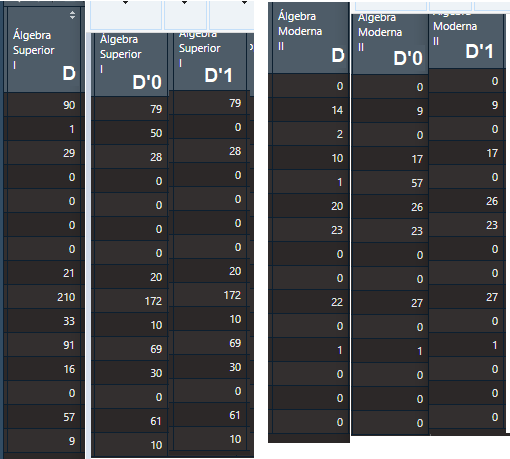
\includegraphics[scale = 1]{Ej_gmm} %width=\textwidth
%\caption{\textit{Ejemplo de la obtención de D'}}
%\end{figure}

En la \figurename{~\ref{GMM_inicial_final}} se muestran dos histogramas con los datos iniciales y finales, respectivamente. Las líneas verdes corresponden al ajuste con la función \verb@density()@ en \textit{R} y las azules al modelo de mezcla de normales.

\begin{figure}[H]
\centering
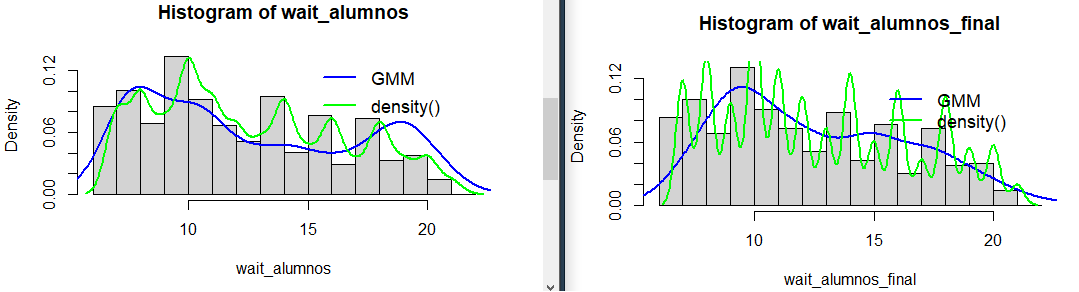
\includegraphics[width=\textwidth]{histograma_y_GMM} %scale = 1
\caption{\textit{Mezcla de normales inicial y final}}\label{GMM_inicial_final}
\end{figure}
